\documentclass[tikz,border=10pt]{standalone}
\usepackage{amsmath,amssymb}
\usepackage{tikz}
\usetikzlibrary{arrows,automata,backgrounds,calendar,chains,decorations,decorations.pathreplacing,decorations.text,fit,matrix,mindmap,patterns,petri,plotmarks,positioning,shadows,shapes,shapes.callouts,shapes.geometric,shapes.misc,spy,trees,calc,intersections,tikzmark,arrows.meta}
\usepackage{xcolor}
\usepackage{pgfplots}
\pgfplotsset{compat=1.16}

% Common math macros from the book
\def\x{\mathbf{x}}
\def\y{\mathbf{y}}
\def\z{\mathbf{z}}
\def\A{\mathbf{A}}
\def\b{\mathbf{b}}
\def\c{\mathbf{c}}
\def\w{\mathbf{w}}
\def\v{\mathbf{v}}
\def\u{\mathbf{u}}
\def\e{\mathbf{e}}
\def\zero{\mathbf{0}}
\def\R{\mathbb{R}}
\def\N{\mathbb{N}}
\def\Z{\mathbb{Z}}
\def\Q{\mathbb{Q}}
\def\st{\text{s.t.}}
\def\vect#1{\mathbf{#1}}
\def\xLP{x^{\mathrm{LP}}}
\def\zLP{z^{\mathrm{LP}}}
\def\xIP{x^{\mathrm{IP}}}

% Common node styles from the book
\tikzset{
    main/.style={circle, draw, fill=gray!20, minimum size=1cm, font=\normalsize},
    dot/.style={circle,fill=blue,minimum size=3pt,inner sep=0pt, outer sep=-1pt},
    vertex/.style={circle,fill=black!25,minimum size=20pt,inner sep=0pt},
    edge/.style={draw,-,thick},
    directed edge/.style={draw,->,>=latex,thick},
}

% Additional macros for 3D/coordinate systems
\newcommand{\xhat}{\hat{\x}}
\newcommand{\yhat}{\hat{\y}}
\newcommand{\zhat}{\hat{\z}}
\newcommand{\ihat}{\hat{\imath}}
\newcommand{\jhat}{\hat{\jmath}}
\newcommand{\khat}{\hat{k}}

\begin{document}
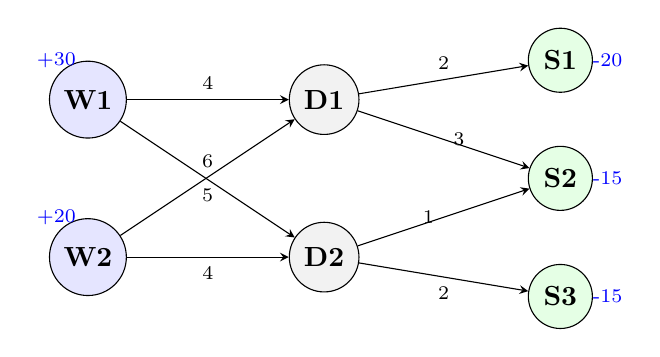
\begin{tikzpicture}[>=stealth, node distance=2cm]

% Warehouses
\node[draw, circle, fill=blue!10] (W1) at (0,2) {\textbf{W1}};
\node[draw, circle, fill=blue!10] (W2) at (0,0) {\textbf{W2}};

% Distribution Centers
\node[draw, circle, fill=gray!10] (D1) at (3,2) {\textbf{D1}};
\node[draw, circle, fill=gray!10] (D2) at (3,0) {\textbf{D2}};

% Stores
\node[draw, circle, fill=green!10] (S1) at (6,2.5) {\textbf{S1}};
\node[draw, circle, fill=green!10] (S2) at (6,1) {\textbf{S2}};
\node[draw, circle, fill=green!10] (S3) at (6,-0.5) {\textbf{S3}};

% Arcs with costs
\draw[->] (W1) -- (D1) node[midway, above] {\scriptsize 4};
\draw[->] (W1) -- (D2) node[midway, below] {\scriptsize 5};
\draw[->] (W2) -- (D1) node[midway, above] {\scriptsize 6};
\draw[->] (W2) -- (D2) node[midway, below] {\scriptsize 4};
\draw[->] (D1) -- (S1) node[midway, above] {\scriptsize 2};
\draw[->] (D1) -- (S2) node[midway, right] {\scriptsize 3};
\draw[->] (D2) -- (S2) node[midway, left] {\scriptsize 1};
\draw[->] (D2) -- (S3) node[midway, below] {\scriptsize 2};

% Supply/demand
\node[blue] at (-0.4,2.5) {\scriptsize +30};
\node[blue] at (-0.4,0.5) {\scriptsize +20};
\node[blue] at (6.6,2.5) {\scriptsize -20};
\node[blue] at (6.6,1) {\scriptsize -15};
\node[blue] at (6.6,-0.5) {\scriptsize -15};

\end{tikzpicture}
\end{document}
